%%%%%%%%%%%%%%%%%%%%%%%%%%%%%%%%%%%%%%%%%%%%%%%%%%%%%%%%%%%%%%%%%%%%%%%%%%%%
% Section 2: Background Information of RapidSmith, RapidSmith2, and Tincr
%%%%%%%%%%%%%%%%%%%%%%%%%%%%%%%%%%%%%%%%%%%%%%%%%%%%%%%%%%%%%%%%%%%%%%%%%%%%
\newpage
\section{Background}

\graphicspath{{./techReportFigures/sec2_background/}}

RapidSmith2 is based on the original RapidSmith project created by Christopher
Lavin as a part of his PhD work at BYU.  It was based on the Xilinx Design
Language (XDL) which provides a human-readable file format equivalent to the
Xilinx proprietary Netlist Circuit Description (NCD) of \textbf{ISE}.  With
RapidSmith, researchers were able to import XDL, manipulate, place, route and export
designs among a variety of design transformations.  The RapidSmith project made
an excellent test bed to try out new ideas and algorithms for FPGA CAD research
because code could quickly be written to take advantage of the APIs available.
RapidSmith also contained packages which could parse/export bitstreams (at the
packet level) and represent the frames and configuration blocks in the provided
data structures. RapidSmith continues to be functional and is still available at
{\color{blue} http://rapidsmith.sourceforge.net/}. There, you will find
documentation, installation instructions, the RapidSmith code base, and a
collection of demo programs demonstrating example CAD tools.

RapidSmith is a great contribution to the FPGA community, but as previously
stated is built upon the XDL interface offered in Xilinx's ISE tools suite.
Unfortunately, Vivado (Xilinx's newest tool suite) does not support XDL. This
makes CAD tools based on XDL incompatible with next-generation Xilinx devices
such as UltraScale and UltraScale+. Instead, Vivado offers a Tcl interface
that can potentially be used to extract Xilinx device and design information.
The ultimate goal of RapidSmith2 is to update the original RapidSmith to support
implementing CAD tools with Vivado designs. The remainder of this section gives
an overview of the required components developed to support Vivado CAD tool
creation in RapidSmith2.

\subsection{Vivado Tool Suite}
In recent years, Xilinx released their new vendor tool for programming FPGAs:
Vivado. Vivado supersedes ISE (the previous tool), and is the only tool suite
that supports the latest Xilinx families such as UltraScale. The most
significant change with Vivado is the introduction of a Tcl interface. Using
Tcl commands, users of Vivado can write Tcl code to script design flows, set
constraints on a design, and perform low-level design modifications. There are
Tcl commands for a variety of useful functions including: finding all tiles in
a device, getting all of the used PIPs in a routed design, and grouping related
cells into a macro. For example, the Tcl command \texttt{[get\_sites -filter
(SITE\_TYPE==SLICEL \&\& !IS\_USED)]} will return a list of all unused SLICEL
sites in the current device. This list could potentially be used to add
additional logic to a design post-route. The Tcl interface is a powerful
addition to the Xilinx tool suite, but suffers some major drawbacks:

\begin {itemize}
  \item Tcl, being an interpreted language, is slow. Compiled or managed runtime
  systems are better options for performance.
  \item Vivado's Tcl interface does not manage memory well. A simple Tcl script
  can cause the memory usage of Vivado to grow indefinitely.
  \item Tcl does not natively support higher-level programming constructs,
  making it more difficult to implement complex algorithms (such as
  PathFinder).
\end{itemize}

\noindent These drawbacks largely motivate using the Tcl interface as an
\textit{extraction} tool, instead of a CAD framework itself. Vivado Tcl scripts
can be used for this purpose.

\subsection{Tincr} \label{sec:tincr}
\texttt{Tincr} is a Tcl plugin to Vivado created by
Brad White as a part of this MS Thesis at BYU. It introduces two useful packages:
\texttt{TincrCAD} and \texttt{TincrIO}. These packages augment Vivado's native Tcl interface with a
set of high-level commands that (a) simplify a variety of Vivado tasks and (b)
add additional functionality to the Tcl interface in the form of new Tcl
commands. \texttt{TincrCAD} focuses on commands for implementing CAD tools
directly in Vivado, and \texttt{TincrIO} focuses on commands for extracting
device and design data from Vivado. \texttt{TincrIO} is especially important
for RapidSmith2 because it demonstrated the feasibility of using
Tcl commands to manipulate Vivado designs outside of Vivado.

\subsection{Vivado Design Interface}
\texttt{Tincr} design extraction was a good start for supporting Vivado designs
in external CAD tools, but it was far from complete and didn't represent several
important aspects of Vivado designs. The \textbf{Vivado Design Interface} (VDI),
a complete Vivado device and design extraction tool, was developed by Thomas
Townsend as a part of his MS Thesis at BYU, and was based on the intial work by
Brad White.
VDI is included with
\texttt{Tincr}, and is available at {\color{blue}
\url{https://github.com/byuccl/tincr}}. It is a  significant contribution for
two reasons in particular:

\begin{enumerate}
  \item VDI defines a set of file formats used to externally represent
  Vivado devices and designs in a general, open-source way.
  
  \item VDI includes Vivado Tcl code to parse and generate design and device
  files.
\end{enumerate}

\noindent VDI is meant to serve as a general-purpose interface into the Vivado
design suite which can be used with \textit{any} CAD tool or framework. It
provides an XDL-alternative for designs implemented in Vivado. Devices are
represented with a XDLRC file and a set of XML files. Designs are represented
with RSCP and TCP checkpoint files. RapidSmith2 uses VDI to interface designs
with the Vivado tool suite.

\begin{figure}[h!]
 \centering
 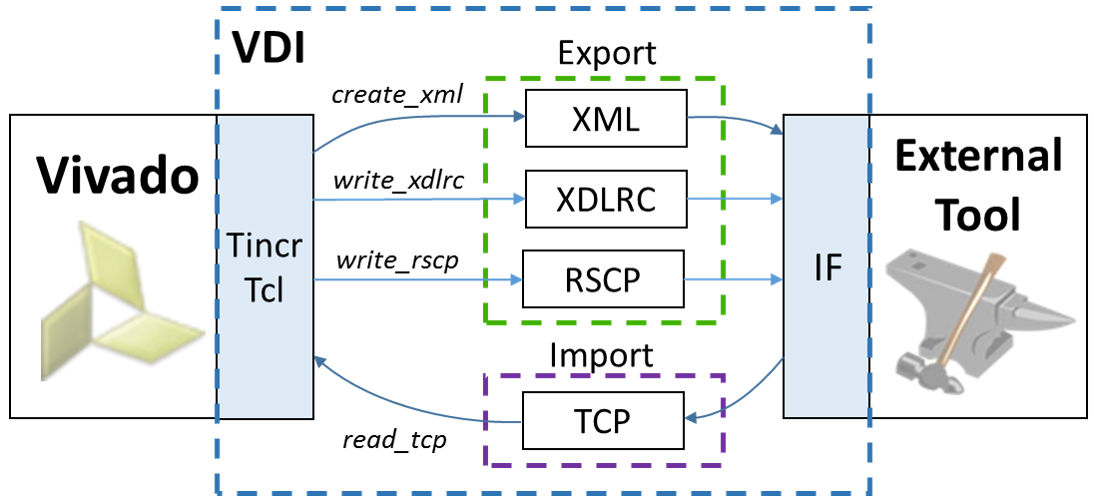
\includegraphics[width=.8\columnwidth]{vdi.png}
 \caption{Components of the Vivado Design Interface (VDI)}
 \label{fig:vdi}
\end{figure}

\subsection{RapidSmith2}

The RapidSmith framework has helped researchers create several different CAD
tools targeting Xilinx devices. Due to the format of XDL however, these CAD
tools always operate at site boundaries. This makes it difficult to explore sub-site CAD
algorithms that work explicitly with sub-site components (i.e. BELs, site PIPs,
etc.) such as packers. Travis Haroldsen was interested in exploring packing
algorithms for Virtex6 devices, and so began the creation of RapidSmith2 as a
part of his PhD work at BYU.
RapidSmith2 updated the internal data structures of RapidSmith to the BEL and cell-level, allowing
algorithms to have finer grained control over sub-site placement and routing. 
Because it was originally targeting the Virtex6 architecture, the initial
version of RapidSmith2 took as input a XDL netlist, and \textbf{unpacks} the
netlist to its corresponding cells, nets, BELs, and wires. RapidSmith2 has
since been updated to support Vivado designs exported through VDI (achieving
the original goal of this work). The remainder of this document details
important aspects of RapidSmith2 to help researchers quickly develop
experimental CAD tools for their research.

\subsection{RapidSmith2 Usage Model and Structure}
The usage model for RapidSmith2 is shown in \autoref{fig:UsageModels}.  As can be
seen, a design can be exported from Vivado at multiple different points in the
Vivado design flow through VDI. In each case, Tincr is used to export a
RapidSmith Checkpoint (RSCP)) which can then be imported into RapidSmith2.  At
those same points in the design flow, RapidSmith2 can export a Tincr Checkpoint
(TCP) which can then be imported back into Vivado. Thus, a complete solution
involves Vivado, Tincr, and RapidSmith2.

\begin{figure}[htb]
\centering
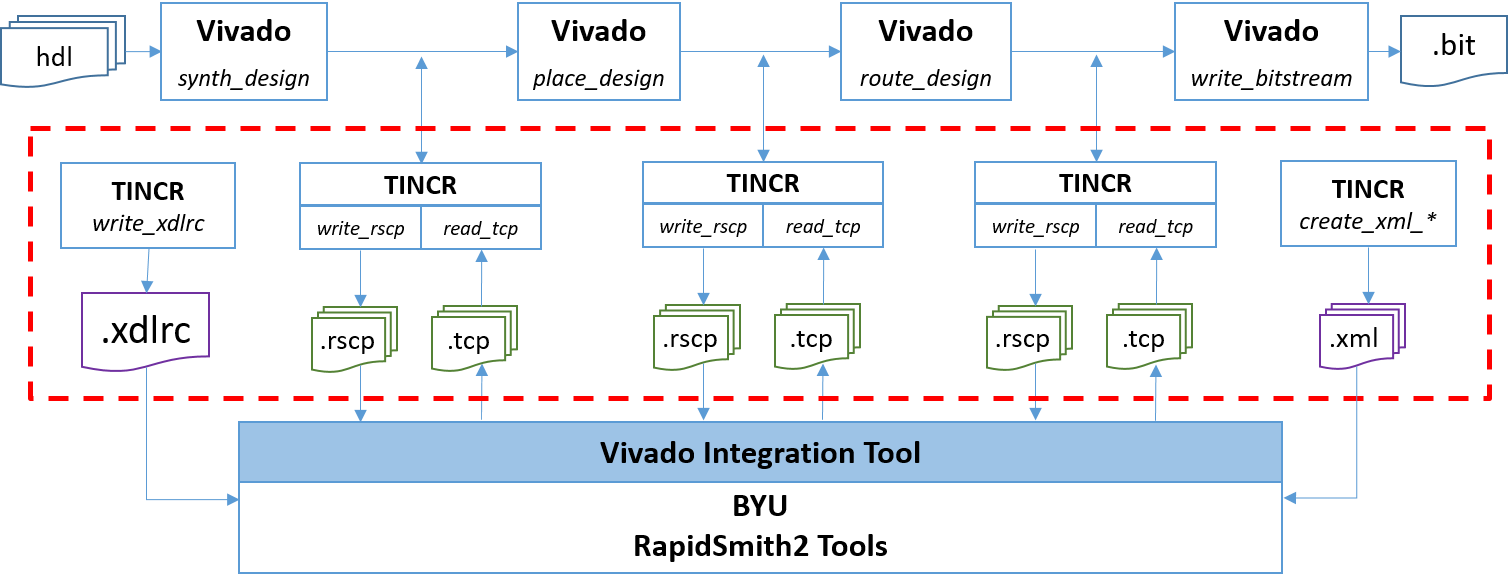
\includegraphics[width=\columnwidth]{usageModel.png}
\caption{Vivado and RapidSmith2 Usage Model}
\label{fig:UsageModels}
\end{figure}

\subsection{Publications and Theses}
Several publications and theses have been accepted as a result of this work.
They are listed here for those who are interested in learning more about RapidSmith2,
\texttt{Tincr}, and VDI.

\begin{enumerate}
  \item B. White. (2014) Tincr: Integrating Custom Cad Tool Frameworks With the
  Xilinx Vivado Design Suite. [Online]. Available:
  http://scholarsarchive.byu.edu/etd/4338/ ix, 6, 92
  
  \item B. White and B. Nelson, “Tincr A Custom CAD Tool Framework for Vivado,”
  in ReConFigurable Computing and FPGAs (ReConFig), 2014 International
  Conference on. IEEE, Dec. 2014. 3, 12 
   
  \item T. Haroldsen, B. Nelson, and B. Hutchings, “Rapidsmith 2: A Framework
  for BEL-Level CAD Exploration on Xilinx FPGAs,” in Proceedings of the 2015
  ACM/SIGDA International Symposium on Field-Programmable Gate Arrays. ACM,
  2015, pp. 66–69. 3, 17
  
  \item  T. Haroldsen, B. Nelson, and B. Hutchings, “Packing a Modern Xilinx
  FPGA Using RapidSmith,” in ReConFigurable Computing and FPGAs (ReConFig),
  2016 International Conference on. IEEE, 2016, pp. 1–6. 17
  
  \item T. Townsend and B. Nelson, “Vivado Design Interface: An Export/Import
  Capability for Vivado FPGA Designs ” in Field Programmable Logic and
  Applications (FPL), 2017 27th International Conference.
  
  \item Townsend, Thomas James, "Vivado Design Interface: Enabling CAD-Tool
  Design for Next Generation Xilinx FPGA Devices" (2017). All Theses and
  Dissertations. 6492. http://scholarsarchive.byu.edu/etd/6492 
\end{enumerate}

% \subsection{RapidSmith vs. RapidSmith2}
% \subsubsection{What Was The Original RapidSmith?}
% The original RapidSmith was written by Christopher Lavin as a part of his PhD
% work at BYU.  It was based on the Xilinx Design Language (XDL) which provides a
% human-readable file format equivalent to the Xilinx proprietary Netlist Circuit
% Description (NCD) of ISE.  With RapidSmith, researchers were able to import
% XDL/NCD, manipulate, place, route and export designs among a variety of design
% transformations.  The RapidSmith project made an excellent test bed to try out
% new ideas and algorithms for FPGA CAD research because code could quickly be
% written to take advantage of the APIs available.
% 
% RapidSmith also contained packages which could parse/export bitstreams (at the
% packet level) and represent the frames and configuration blocks in the provided
% data structures.  In this regard, RapidSmith did not include any proprietary
% information about Xilinx FPGAs that is not publicly available.
% 
% RapidSmith continues to be functional and is still available at the
% SourceForge.net website.  There, you will find documentation, installation
% instructions, the RapidSmith code base, and a collection of demo programs based
% on it.
% 
% \subsubsection{What is RapidSmith2?}
% With the announced end of ISE (with the Virtex7 family of parts being the last
% family to be supported by ISE), there was no path forward to newer parts using
% RapidSmith.  This is because XDL is not available with Vivado. With
% Vivado, however, Xilinx has provided an extensive Tcl scripting capability which 
% initially looked as if it could provide a similar capability to that provided by
% XDL in terms of accessing both Vivado's design and device data and in terms of
% creating and modifying Vivado designs.  However, as described above, Vivado's
% Tcl is limited by speed and memory challenges.
% The development of RapidSmith2 consisted of three parts.
% 
% \subsubsection{Tincr: Integrating Custom CAD Tool Frameworks with the Xilinx 
% Vivado Design Suite} \label{sec:tincr}
% 
% In the first part, the Vivado Tcl capability was investigated to ensure that,
% indeed, it did provide the needed ability to access design and device data and
% export that to external tools such as RapidSmith.  This resulted in the Tincr
% project, led by Brad White as a part of his MS work at BYU, with Thomas
% Townsend making additions as a part of his research.
% 
% Tincr is a Tcl-based library of routines which (a) provide a variety of
% functions to simply make working with Vivado via Tcl easier, (b) provide a way
% to export all the data associated with a Vivado design into what is called a
% Tincr Checkpoint (TCP), (c) provide a way to reimport Tincr Checkpoints back
% into Vivado, and (d) access device data from Vivado and output that data in the
% form of XDLRC files (these are the files which XDL used to describe devices and
% are necessary for RapidSmith and RapidSmith2 to understand the structure of and the
% resources available for use in a given Xilinx part).  Tincr is available at 
% \href{https://github.com/byuccl/tincr}{\color{blue}https://github.com/byuccl/tincr}.
% Tincr is described in two publications:
% 
% \begin{quotation}B. White and B. Nelson, "Tincr � A custom CAD tool framework
% for Vivado," 2014 International Conference on ReConFigurable Computing and FPGAs (ReConFig14),
% Cancun, 2014, pp. 1-6, DOI: 10.1109/ReConFig.2014.7032560
% 
% White, Brad S., "Tincr: Integrating Custom CAD Tool Frameworks with
% the Xilinx Vivado Design Suite" (2014), BYU Scholars Archive, Paper 4338. 
% \\URL:http://scholarsarchive.byu.edu/etd/4338
% \end{quotation}
% 
% \subsubsection{RapidSmith2: A Framework for BEL-Level CAD Exploration on Xilinx FPGAs}
% The second part of the development of RapidSmith2 was to add a new layer of design
% representation to RapidSmith which more closely matches that of Vivado.  This
% was done as a part of his PhD work by Travis Haroldsen at BYU.  As of this
% writing, one paper on RapidSmith2 has appeared:
% 
% \begin{quotation}Travis Haroldsen, Brent Nelson, and Brad Hutchings, “RapidSmith
% 2:
% A Framework for BEL-Level CAD Exploration on Xilinx FPGAs�, Proceedings of the
% 2015 ACM/SIGDA International Symposium on Field-Programmable Gate Arrays,
% February 2015, Monterey CA, pp. 66-69, DOI: 10.1145/2684746.2689085.
% \end{quotation}
% 
% \subsubsection{Vivado and RapidSmith2 Integration}
% The third part of the development of RapidSmith2 was to create the ability to export
% designs from Vivado and into RapidSmith2 and, correspondingly, to import RapidSmith2 data back
% into Vivado.  This was completed during 2016, largely by Thomas Townsend
% as an MS student at Brigham Young University.  The initial
% public release of RapidSmith2 was made in January 2017 once that piece was in place.
% 
% \subsubsection{What is All This About XDL and XDLRC and How Does RapidSmith2 Fit Into
% That?} 
% The Xilinx ISE tools had the capability to export XDL and XDLRC files which
% RapidSmith used: 
% \begin{itemize}
%   \item An XDLRC file was a complete description of a given Xilinx FPGA,
%   describing every tile, every switchbox, every wire segment, and every PIP in
%   the part.  RapidSmith was able to process this information and create a device
%   representation for use in support of CAD tools such as placers and routers.
%   \item An XDL file was a textual representation of an NCD file (a user design).
%   It described the user design as a collection of \cls{Instances} and \cls{Nets}. Instances
%   correspond to things like {SLICEs}, {BRAMs}, {DSP48s}, and {IOBs}.  Instances could be
%   placed onto \cls{Sites}. Additionally, Nets in XDL consisted of a list of
%   \cls{Pins} (their logical connections) and an optional list of \cls{PIPs} (their physical
%   routing connections).
% \end{itemize}
% In Vivado, however, designs are described as a collection of \cls{Cells} where a Cell
% corresponds to things like LUTs, flip flops, etc.  A Cell may be placed
% onto a \cls{BEL} object such as an ALUT or a BFF.  RapidSmith2 contains a new layer of
% hierarchy in its design and device descriptions where Cells and BELs are first-class objects and
% design manipulation is all done at the Cell/BEL level.
% 
% Also, Vivado Nets are described using directed routing strings rather than lists
% of PIPs.  RapidSmith2 also contains a set of new classes to enable the representation
% and manipulation of Nets in a format compatible with these routing strings.
% 
% Thus, using RapidSmith2, design manipulation is now done at the level of Cells and BELs
% and importing/exporting designs to/from Vivado is now fully supported.
% 
% \subsection{RapidSmith2 Usage Model and Structure}
% The usage model for RapidSmith2 is shown in \autoref{fig:UsageModels}.  As can be
% seen, a design can be exported from Vivado at multiple different points in the
% Vivado design flow.  In each case, Tincr is used to export a RapidSmith
% Checkpoint (RSCP)) which can then be imported into RapidSmith2.  At those same points in
% the design flow, RapidSmith2 can export a Tincr Checkpoint (TCP) which can then be
% imported back into Vivado.
% Thus, a complete solution involves Vivado, Tincr, and RapidSmith2.
% 
% \begin{figure}[htb]
% \centering
% 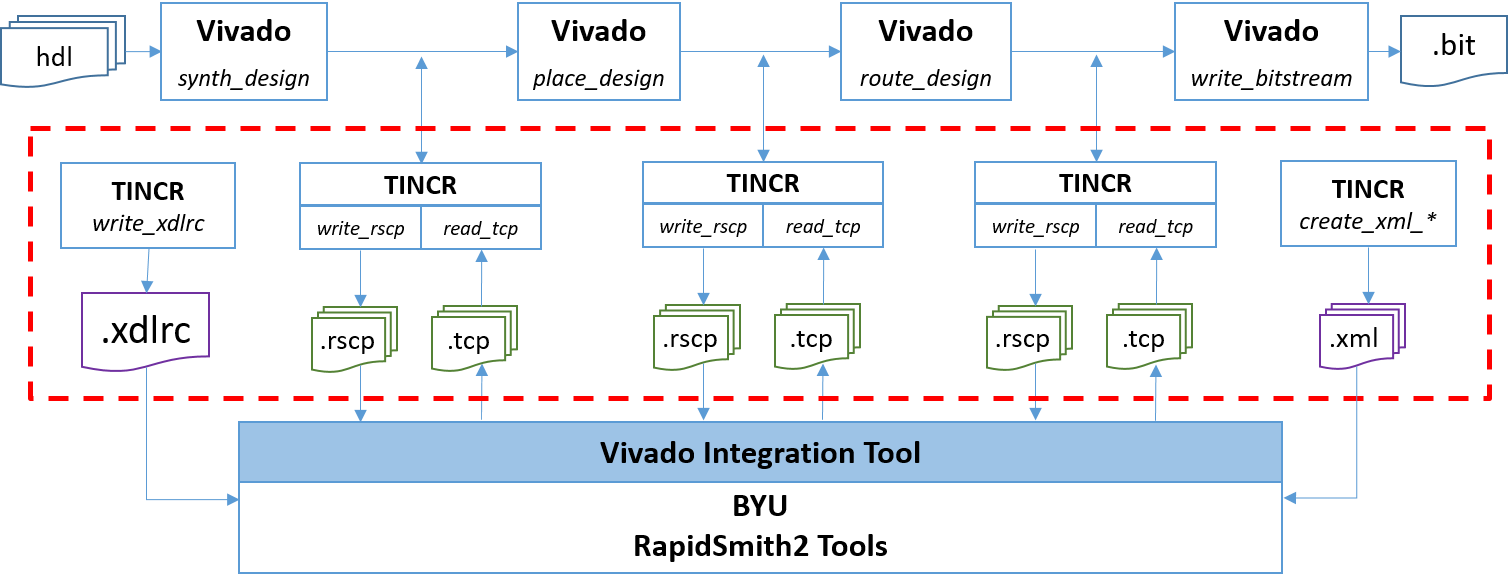
\includegraphics[width=\columnwidth]{usageModel.png}
% \caption{Vivado and RapidSmith2 Usage Model}
% \label{fig:UsageModels}
% \end{figure} 
